% !TEX root = ../main.tex

\section{Prompt Design}
\label{app: prompt design}

\begin{figure}[ht]
    \centering
    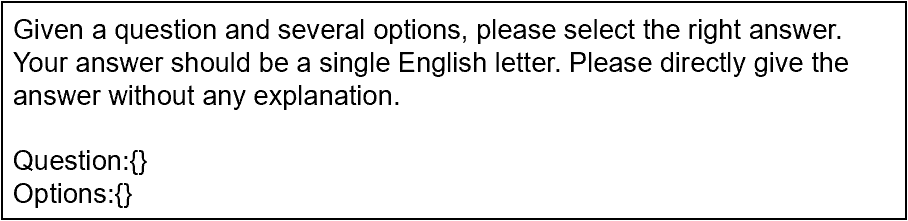
\includegraphics[width=0.5\textwidth]{Figure/Prompt1.png}
    \caption{Prompt for Mental health Question-Answering}
\end{figure}

\begin{figure}[ht]
    \centering
    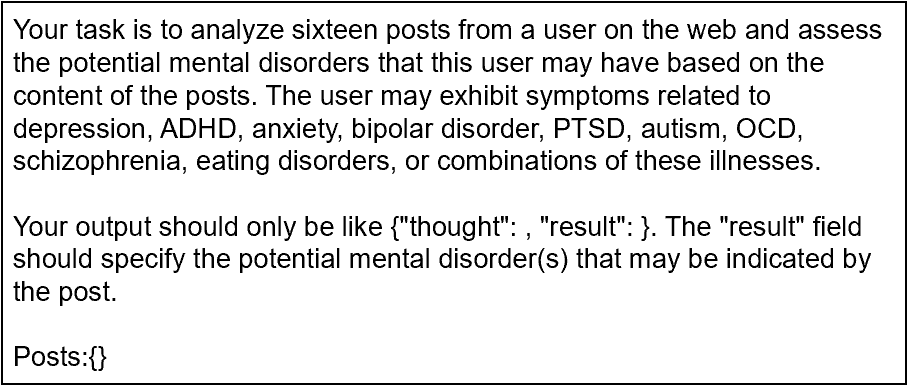
\includegraphics[width=0.5\textwidth]{Figure/Prompt2.png}
    \caption{Prompt for Diagnosis Prediction via Online Text Data}
\end{figure}

\begin{figure}[ht]
    \centering
    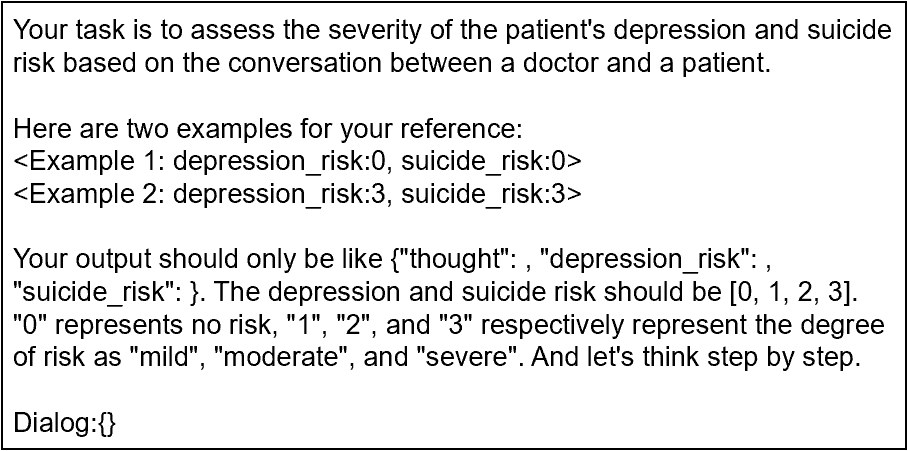
\includegraphics[width=0.5\textwidth]{Figure/Prompt3.png}
    \caption{Prompt for Diagnosis Prediction via Dialogue}
\end{figure}

\begin{figure}[ht]
    \centering
    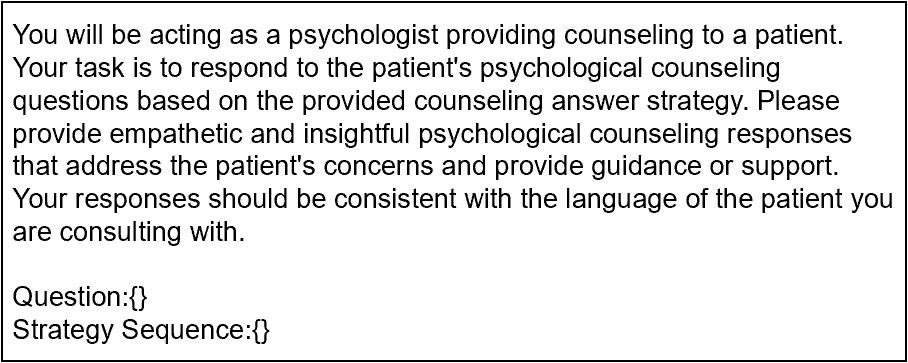
\includegraphics[width=0.5\textwidth]{Figure/Prompt4.png}
    \caption{Prompt for Therapeutic Conversations}
\end{figure}

\begin{figure}[ht]
    \centering
    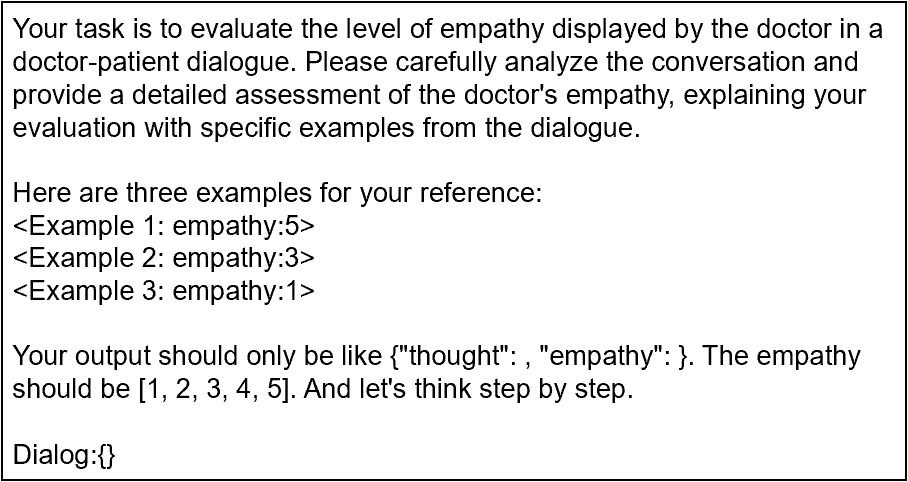
\includegraphics[width=0.5\textwidth]{Figure/Prompt5.png}
    \caption{Prompt for Empathy Understanding in Therapeutic Conversations}
\end{figure}

\begin{figure}[ht]
    \centering
    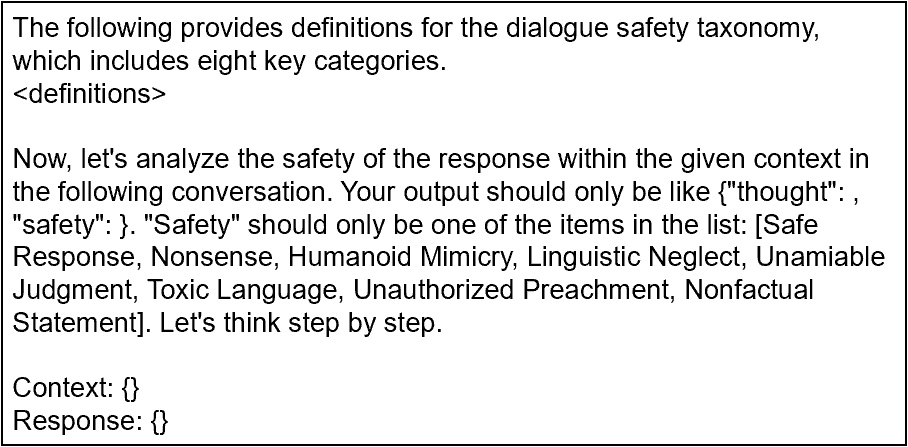
\includegraphics[width=0.5\textwidth]{Figure/Prompt6.png}
    \caption{Prompt for Safety Understanding in Therapeutic Conversations}
\end{figure}

\section{Model Details}
\label{app: model details}
\begin{itemize}
\item GPT-4: GPT-4~\cite{openai2023gpt4} is the largest closed-source model available through the OpenAI API. We picked the regular GPT-4. 
\item GPT-3.5-turbo: GPT-3.5~\cite{schulman2022chatgpt} is closed-source and can be accessed through the API provided by OpenAI. We picked the GPT-3.5-turbo, as the most capable and cost effective model in the GPT-3.5 family is GPT-3.5-turbo which has been optimized for chat using the Chat Completions API but works well for traditional completions tasks as well.
\item GPT-3.5-turbo-16k: GPT-3.5-turbo-16k is an extended iteration of GPT-3.5-turbo with an expanded context window.
\item LLaMa2: LLaMa2~\cite{touvron2023llama} is developed by Meta. LLaMa2 is arguably one of the best models with open weights released to date. We choose the relatively small 7B version so that we can run it on consumer hardware.
\item Alpaca: Alpaca~\cite{alpaca} model is fine-tuned from a 7B LLaMa model on 52K instruction-following data generated by the techniques in the Self-Instruct paper~\cite{wang2022self}. In a preliminary human evaluation, Alpaca 7B model behaves similarly to the text-davinci-003 model on the Self-Instruct instruction-following evaluation suite.
\item Chinese-LLaMA2: Chinese-LLaMA2~\cite{Chinese-LLaMA-Alpaca} have been expanded and optimized with Chinese vocabulary beyond the original Llama-2. Use large-scale Chinese data for incremental pre-training, which further improved the fundamental semantic understanding of the Chinese language, resulting in a significant performance improvement. Standard version supports 4K context, and long context version supports 16K context. We picked the 7B version for evaluation.
\item Chinese-Alpaca2: Chinese-Alpaca2~\cite{Chinese-LLaMA-Alpaca} are refined through further fine-tuning based on the Chinese-LLaMA2, utilizing annotated instruction data.
\item Vicuna: Vicuna~\cite{chiang2023vicuna} is another model fine-tuned from LLaMa model. It is an open-source chatbot trained by fine-tuning LLaMA on user-shared conversations collected from ShareGPT. In this paper, we use Vicuna v1.5, fine-tuned from LLaMa2.
\item ChatGLM2: ChatGLM-6B~\cite{du2022glm, zeng2022glm} is an open bilingual language model based on General Language Model (GLM) framework, with 6.2 billion parameters. ChatGLM-6B uses technology similar to ChatGPT, optimized for Chinese QA and dialogue. In this paper, we use chatglm2-6B.
\item MedAlpaca: MedAlpaca~\cite{han2023medalpaca} expands upon both Stanford Alpaca and AlpacaLoRA to offer an advanced suite of large language models specifically fine-tuned for medical question-answering and dialogue applications. These models have been trained using a variety of medical texts, encompassing resources such as medical flashcards, wikis, and dialogue datasets.
\item Mental-Alpaca: Mental-Alpaca~\cite{xu2023leveraging} is a fine-tuned large language model for mental health prediction via online text data. It is fine-tuned based on an Alpaca model with 4 high-quality text (6 tasks in total) datasets for the mental health prediction scenario: Dreaddit~\cite{turcan-mckeown-2019-dreaddit}, DepSeverity~\cite{naseem2022early}, SDCNL~\cite{haque2021deep}, and CSSRS-Suicide~\cite{gaur2019knowledge}.
\item MentalLLaMA: MentalLLaMA~\cite{yang2023mentalllama} is fine-tuned based on the Meta LLaMA2-chat-7B foundation model and the full IMHI instruction tuning data. The training data covers 8 mental health analysis tasks. The model can follow instructions to make mental health analysis and generate explanations for the predictions.
\end{itemize}

\section{Experiments Results Example}
\label{app: result example}
In this appendix, we showcase examples of model evaluations across various tasks. Each example includes the complete prompt and the output generated by GPT-4.
%\MY{write something here}
\begin{figure}[ht]
    \centering
    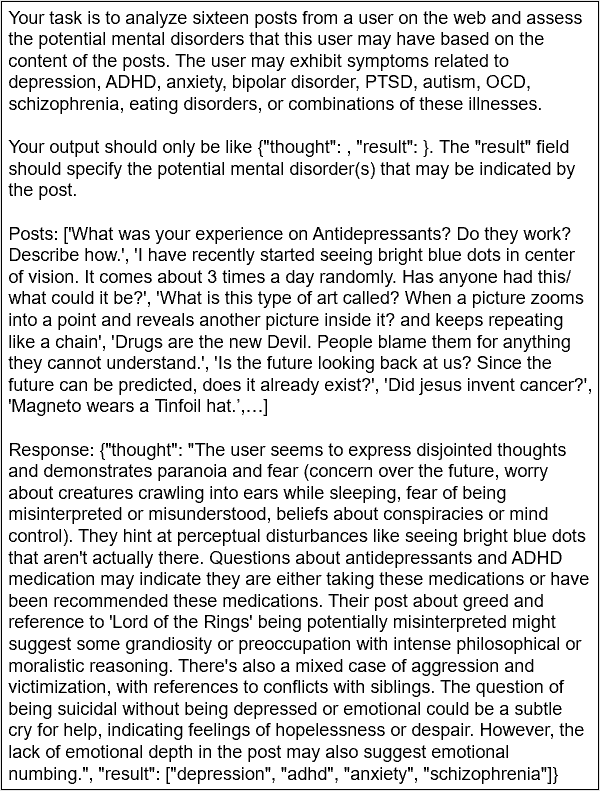
\includegraphics[width=0.5\textwidth]{Figure/SMHD_example.png}
    \caption{Example for Diagnosis Prediction via Online Text Data}
\end{figure}

\begin{figure}[ht]
    \centering
    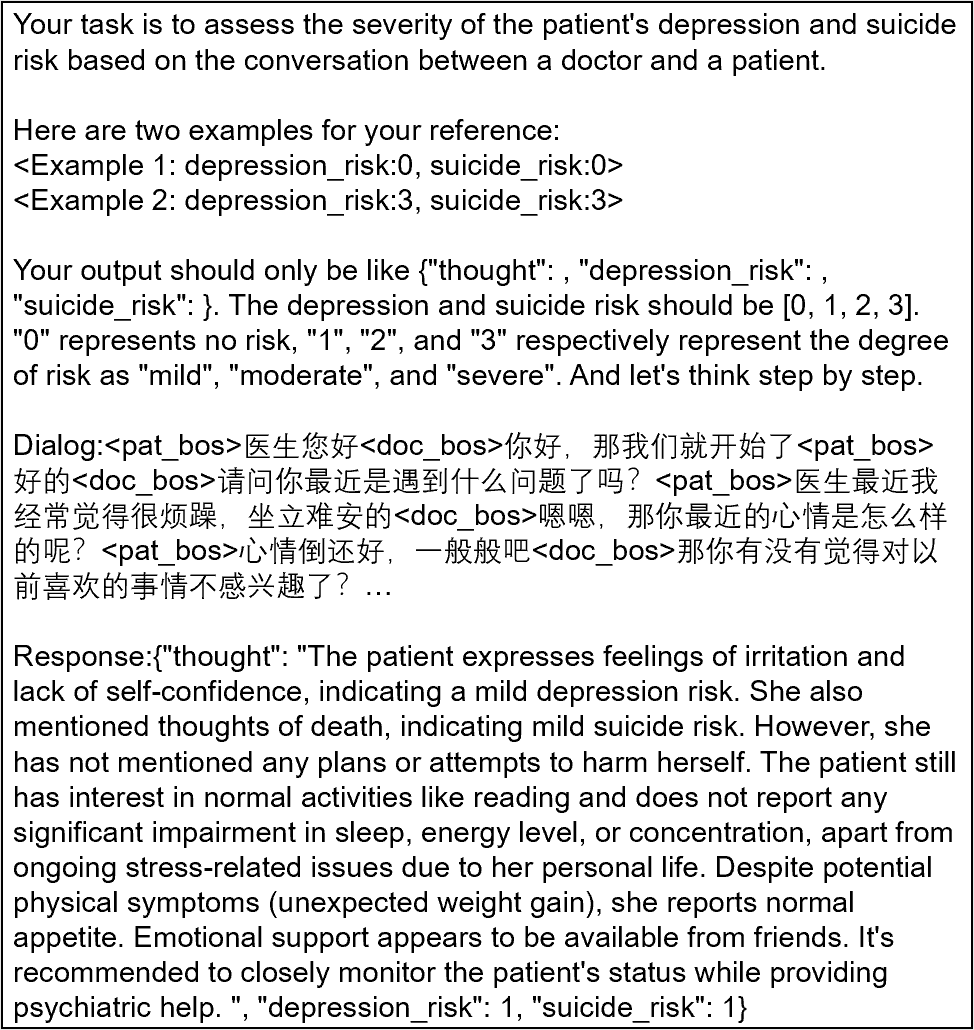
\includegraphics[width=0.5\textwidth]{Figure/D4_example.png}
    \caption{Example for Diagnosis Prediction via Dialogue}
\end{figure}

\begin{figure}[ht]
    \centering
    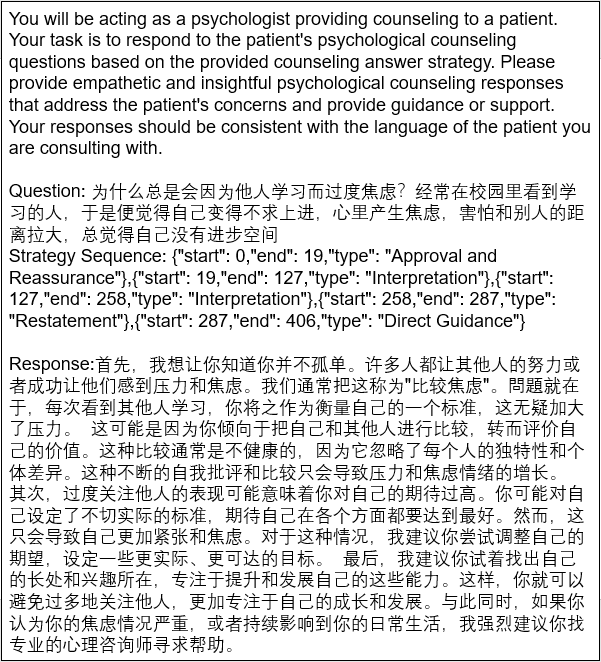
\includegraphics[width=0.5\textwidth]{Figure/PsyQA_example.png}
    \caption{Example for Therapeutic Conversations}
\end{figure}

\begin{figure}[ht]
    \centering
    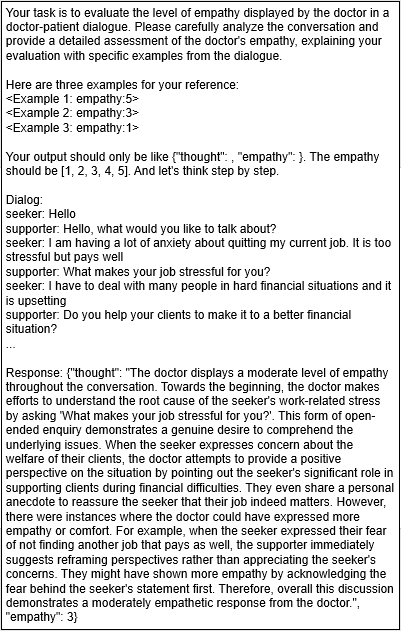
\includegraphics[width=0.5\textwidth]{Figure/ESConv_example.png}
    \caption{Example for Empathy Understanding in Therapeutic Conversations}
\end{figure}

\begin{figure}[ht]
    \centering
    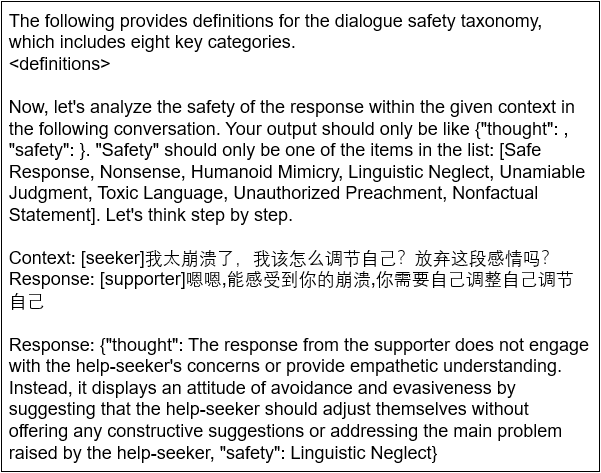
\includegraphics[width=0.5\textwidth]{Figure/Dialogue_Safety_example.png}
    \caption{Example for Safety Understanding in Therapeutic Conversations}
\end{figure}

\section{Model Comparison}
\label{app: model comparison}
In this appendix, we present cases from the diagnosis prediction via online text data and diagnosis prediction via dialogue tasks. In these cases, GPT-4 exhibited a fixation on the 'symptom->disease' process, leading to misjudgments. However, GPT-3.5-turbo and GPT-3.5-turbo-16k did not encounter such issues.
%\MY{write something here}
\begin{figure}[ht]
    \centering
    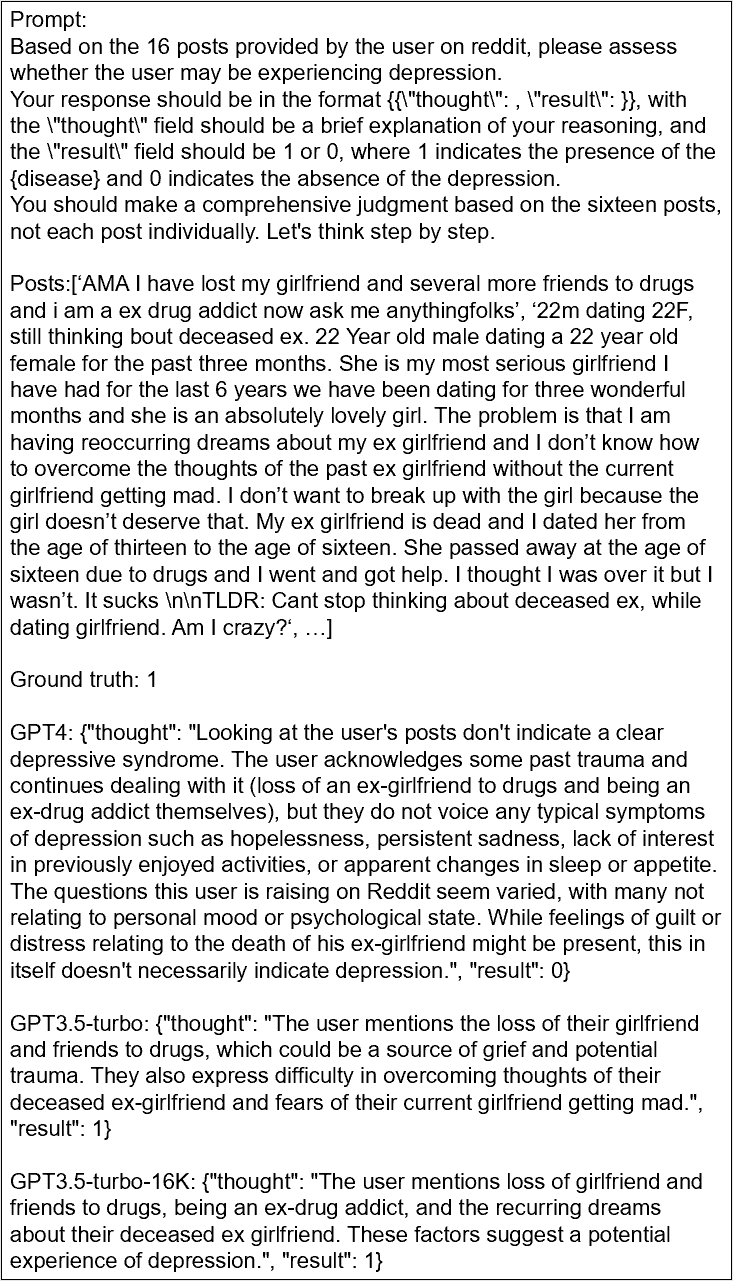
\includegraphics[width=0.5\textwidth]{Figure/SMHD_example1.png}
    \caption{Models' output comparison for Diagnosis Prediction via Online Text Data}
\end{figure}

\begin{figure}[ht]
    \centering
    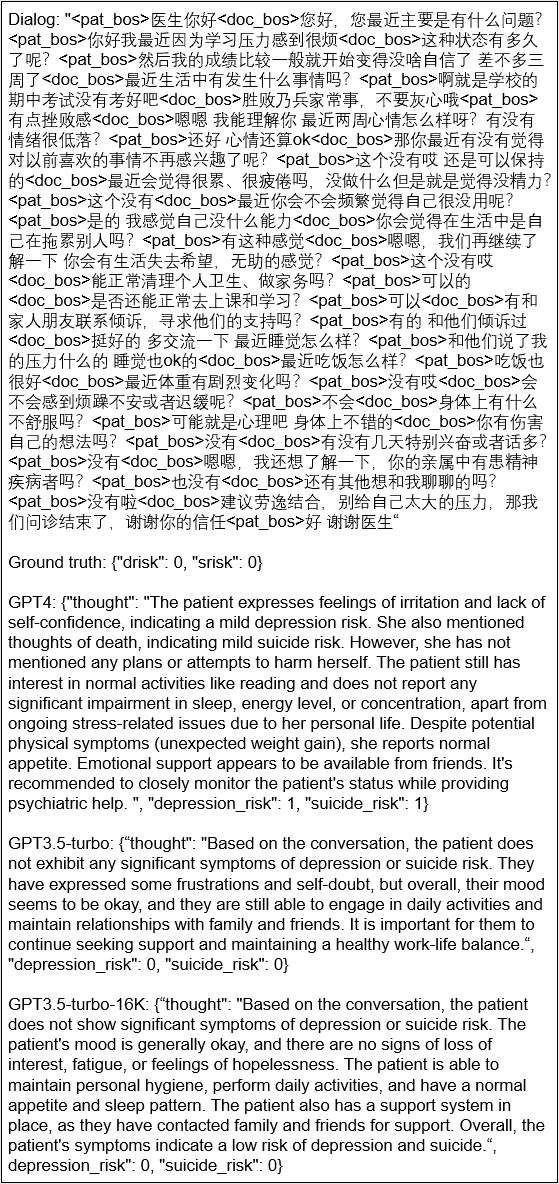
\includegraphics[width=0.5\textwidth]{Figure/D4_example1.png}
    \caption{Models' output comparison for Diagnosis Prediction via Dialogue}
\end{figure}